\chapter{Grundlagen}

\section{Roboter-Mensch-Kollaboration}
\label{sec:roboter-mensch-kollaboration_gru}

Man unterscheidet die Arbeiten mit einem Roboter unter mehrere Arten.
Roboter die mit anderen Robotern gleichzeitig arbeiten nennt man Kooperation zwichen Robotern.
Der Mensch ist in diesem Arbeitsumfeld nicht dabei und kann nur von außen einfluss nehmen.
\\\\
Als nächstes gibt es die Kollaboration zwichen dem Roboter und dem Mensch. 
Hier wird auch eine Unterteilung vorgenommen die unterschiedliche Richtlinien erfordern.

\begin{itemize}
\item Sicherhaltshalt, wenn der Mensch den Kollaborationsraum betritt.
\item Dauerhafte Überwachung des abstands zwichen Mensch und Roboter, der mit reduzierter geschwindigkeit arbeitet.
\item Verminderte Geschwindigeit. Führung des Roboters durch den Mensch. Sensoren erfassen die kräfte, die vom Menschen ausgeführt werden und übertragen sie auf den Roboter.
\item Beschränkung der im Roboter ausgeführten Energie. Überwachung des Roboters auf Kollision und sofortigem Stop
\end{itemize}

\subsection{Richtlinien}
\label{kol_richtlinien_gru}

In so gut wie allen fällen sind Roboter in der Industrie in einem extra abgesicherten Bereich umzäunt, damit kein Arbeiter sich verletzen kann. Diese Robote sind umhaust. Es ist nicht möglich in einem gemeinsamen Arbeitsbereich zu kollaborieren. 
Damit Menschen im Arbeitsbereich vom Robotern Arbeiten dürfen müssen diese Roboter bestimmte Sicherheitsrichtlinien entsprechen.
Der Roboter darf unter keinen Umständen eine Lebensbedrohliche gefahr darstellen. Die Norm ISO 10218

\section{UR5 Roboter}
\label{sec:ur_robot_gru}

Die Dänische Firma Universal Robots hat den leichten Ur5 und mittelgroßen Ur10 Roboter hergestellt mit erfüllbaren Normen um mit diesem Roboter zu kollaborieren. Man kann sich im laufenden Betrieb in der Nähe aufhalten um Wegpunkte zu Teachen oder auch gleichzeitig an einem Werkstück zu arbeiten. 

\subsection{Kinematik}
\label{ur_eigenschaften_gru}

\begin{figure}[ht]
  \centering
    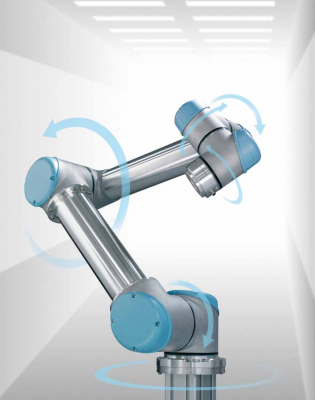
\includegraphics[width=0.8\textwidth]{pic/ur5_robot.png}
      \caption[UR5 Roboter]{Abbildung zeigt den UR5 Roboter von universal Robots}
      \label{fig:schnittstellen_schichten}
\end{figure}

Der Roboter besitzt 6 Gelenke die ihm ermöglichen einen 360° Arbeitsbereich mit einem Radius von ca 85cm zu ermöglichen. Gesteuert wird er von einem Linux Rechner, der sich in der Nähe befindet. 
Die Festplatte für das System ist eine Speicherkarte, die leicht ausgetauscht werden kann.
\\\\
Um den Rechner anzusprechen existiert bei lieferung ein Touch Tablet, das für das Linux System den Visuellen Output gibt. bei Start wird auch automatisch die Software für den Roboter gestartet. Die Software nennt sich Polyscope und wurde in Java geschrieben. Diese Software verbindet sich per TCP/IP auf den URController. Ein Server Programm das die Schnittstelle von dem Linux System zu dem Roboter Controller auf dem Rechner Herstellt.
\\\\
Die Polyscope Software läuft im normalen Modus und den Administrativen Modus. Der Normale Modus ermöglicht es Programme zu erstellen, laufen zu lassen und Grundeinstellungen vorzunehmen. Außerdem kann ein Software Update der Polyscope Software gemacht werden.

\subsection{Peripherie}
\label{ur_update_gru}

Zwei Arten von Updates sind hier zu unterscheiden. Zum einen kann das Linux System geupdatet werden. Auf normalem wege über den Packetmanager des Systems, oder wenn man das neuste Image von Universal Robots runterläd und dann das System neu aufspielt. Hier ist jedoch zu beachten, dass dabei alle Daten verloren gegangen werden. Deshalb sollte eine Datensicherung vorgenommen werden. Wie dies geschieht wird im darauf folgenden Unterkapitel beschrieben(\ref{ur_datensicherung_gru}).
\\\\
Updates für dem Roboter müssen allerdings manuell gemacht werden. Hierfür müssen die aktuellen Updates von der Homepage von Universal Robots runtergeladen werden. Die Update-Datei muss mit der dateiendung .urup auf einen USB Stick mit einem FAT32 Dateisystem abgelegt werden.\\\\
Nachdem der USB Stick an das Linuy System angeschlossen ist, kann von der Polyscope Software das Update ausgeführt werden. Einstellungen->Updates.\\
Im Administrativen Modus können nach dem Update die Firmware's der einzelnen Gelenkcontroller geupdatet werden. Die werden im Update mitgeliefert. Die einzelnen Schritte sind in den Dokumentationen beiliegend auf der CD zu finden.

\subsection{Datensicherung}
\label{ur_datensicherung_gru}

Die Daten des Roboters sind abgelegt in root verzeichniss unter 

\begin{lstlisting}[caption={Pfade Der Ur5 Relevanten Dateien}, label=lst:ur5data ,captionpos=b] 
/root/.urcontrol    #Konfigurationsdateien des Ur5Roboters
/programs   		#alle geschriebenen Programme unter Polyscope
\end{lstlisting}

Es ist möglich die Dateien per USB Stick zu sichern oder über Programme wie ``SCP'' über das Netzwerk zu Kopieren.

\section{Programmierschnittstellen vom UR5}
\label{sec:programm_api_uebersicht_gru}

Der Ur5 Roboter kann auf drei Ebenen angesprochen werden.\\

\begin{itemize}
\item Polyscope
\item URscript
\item C-Api
\end{itemize}

\begin{figure}[ht]
  \centering
    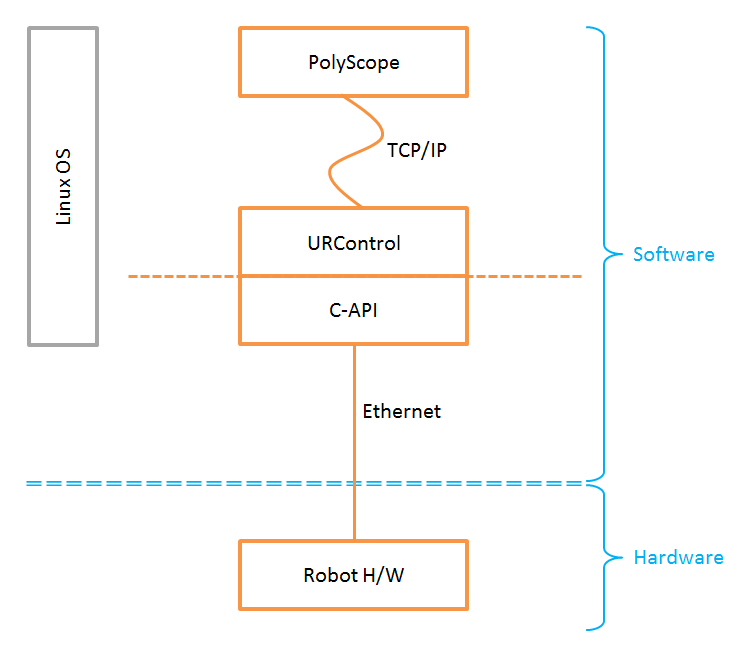
\includegraphics[width=0.8\textwidth]{pic/ur_programming_levels.png}
      \caption[Schichten der Software Schnittstellen]{Übersicht über die
      Schichten der bestehenden Software Schnittstellen des Ur5 Roboters}
      \label{fig:schnittstellen_schichten}
\end{figure}

\section{Kriterien für die Bewertung der Schnittstellen}
\label{sec:criterias_of_solutions_kon}

Die Schnittstellen werden wie folgt bewertet:

\begin{itemize}
\item Programmierbarkeit
\item Interaktion mit Programm,
\item Möglichkeit zu Debuggen und Testbarkeit
\item Aufwendung
\end{itemize}

Wie schwer ist es ein Programm für die einzelnen Schnittsellen zu entwickeln.
Kann der Mensch das Programm Intuitiv bedienen? Wichtig hierbei ist, dass der Mensch mit dem Roboter Kommunizieren kann. Dies geschieht am besten, wenn der Mensch nicht Kryptisch was eingeben muss. Der Mensch braucht Anwenderfreundliche Programme.
\\\\
Beim Entwickeln von Programmen ist es wichtig, dass der Entwickler Fehler im Programm entdeckt um diese schnell zu beheben.
Je Größer und Komplexer das Programm wird, desto schwieriger wird es Fehler zu entdecken.


\section{URControl}
\label{sec:ur_control_gru}

Der URController eine Server Anwendung die auf dem Rechner des Roboters läuft. 
Dieser Controller dient als Schnittstelle von der Roboter Hardware und Software die den Roboter ansteuern wollen.

\subsection{Konfiguration des URControllers}
\label{urcontrol_rci_gru}

Den URController kann man bevor er gestartet wird in einer Konfigurationsdatei konfigurieren.
Hier werden wichtige Einstellungen vorgenommen, die zu den jeweiligen Modellen der Ur5 oder Ur10 Serie gehören. Folgend ist ein ausschnitt der Konfigurationsdatei zu sehen
\\
\begin{lstlisting}
[Config]
# masterboard_version, 0 = Zero-series, 1 = One-series, 
# 3 = Pause function enabled, 4 = first cb2 version, 5 = ur10 support added
masterboard_version = 4
dump_bytecode_on_exception = 1

[Hardware]
controller_box_type = 2 # 1=CB1, 2=CB2UR5, 3=CB2UR10
robot_type = 1  # 1=UR5, 2=UR10
robot_sub_type = 1
\end{lstlisting}

\subsection{Echtzeit Schnittstelle}
\label{urcontrol_rci_gru}

Die Echtzeit Schnittstelle ist eine TCP Schnittstelle, die im 125Hz Takt Nachrichten an die Clients sendet. Diese Schnittstelle empfängt keine Daten von den Clients. Diese Nachrichten müssen von den Clients analysiert und zerlegt werden. Die Daten werden in einer bestimmten form gesendet

TODO !! listing echtzeit schnittstelle

Die Client Anwendung muss nun dieses Packet parsen(Parser: Informationen zerlegen und entsprechend interpretieren.)
Wie Die einzelnen Packete aussehen sind im Anhang mitgeliefert
Für die Programmiersprache C wurde ein ein Parser dafür geschrieben.

\subsection{Secondary und Primary Schnittstelle}
\label{urcontrol_spi_gru}

Das Secondary Interface ist eine TCP Schnittstelle, die in einem 60Hz Takt Nachrichten über den Roboter an Verbundene Rechner sendet.
Die Nachrichten beinhalten Informationen wie z.B. den Roboter Status, die Positionen der einzelenen Joints.
Die volle Beschreibung welche Informationen gesendet werden ist im anhang zu finden.

Zusätzlich, kann die Secondary Schnittstelle befehle von Verbundenen Rechnern empfangen. 
Diese Befehle können URScript befehle sein. Ein ganzes Programm aus URScript befehlen oder spezielle zugelassene Befehle die den Roboter Status verändern.

\begin{figure}[ht]
  \centering
    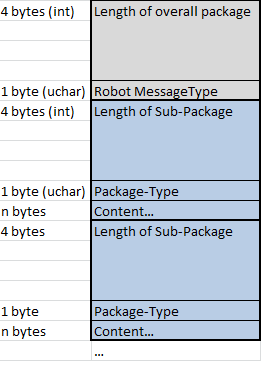
\includegraphics[width=0.5\textwidth]{pic/secondary_datapackage_scheme.png}
      \caption[Schema des Datenpackets gesendet von der Secondary Schnittstelle]{Grobe Darstellung wie das Nachrichten Packet gesendet von der Secondary/Primary Schnittstelle.}
      \label{fig:datascheme_of_secondary_interface}
\end{figure}

\subsection{Polyscope}
\label{urcontrol_polyscope_gru}

Polyscope ist eine Anwendung die auf dem Roboter-Rechner läuft. Die Anwendung verbindet sich per TCP/IP auf den UR Controller und sendet URScript befehler an den Roboter um diesen zu steuern.
Diese Anwendung wird auf dem Tablet angezeigt. Hierrüber kann man per Touch eingabe ein neues .URP Programm erstellen. Dieses Programm wird zur Laufzeit in ein .script umgewandelt.

\section{C-API}
\label{sec:rest_prinzip_gru}

Die C-API ist von dem Hersteller UR eine zur Verfügung gestellte C Library mit einer Header Datei, die etwaige Funktionen der Library erklärt. Die Header Datei enthält nicht alle Funktionen, somit sind nicht alle zugänglich. Die C-API erlaubt es einen eigenen Controller für den Roboter zu entwickeln. Der für den Roboter zur Verfügung gestellte Controller mit der Polyscope Software können aber nicht gleichzeitig laufen. Es schließen sich also die URScriptsprache und ein eigener Controller zunächst aus. Es könnte ein eigener Controller gebaut werden der die Befehle in URScript selbst interpretiert und diese wie bei dem URController ausführt. So könnte man die vorhandene Sprache nehmen und diese sogar erweitern.

\subsection{Kontrollstruktur}
\label{capi_control_loop_gru}	

Die C-API ermöglicht es eine Verbindung zum Roboter zu öffnen und über eigene Funktionen Befehle abzuschicken. Dies erfolgt in einem streng festgelegten Muster. Dieses Muster ist in Abbildung ... TODO !! abilbundsref zu sehen. 
die Funktion robotinterface\_read\_state\_blocking() startet den Bereich in dem Datenabfragen an den Roboter gestellt werden können. Daten wie zb. Temperatur der Motoren, der Stand der Gelenke, die Geschwindigkeit der Gelenke, etc. in der Dokumentation beiliegend zu dieser Arbeit sind alle Daten noch einmal aufgelistet. Nachdem die Daten abgefragt werden, kann mit C-API Functionen Position, Geschwindigkeit und Beschleunigungswerte übermittelt werden, die der Roboter durch seinen Regler auszuführen versucht.\\
Es können jedoch keine Wegpunkte festgelegt werden, die dann automatisch vom Roboter angefahren werden. Dies muss der Entwickler selbst 
berechnen. Es gibt mehrere Verfahren, in dieser Arbeit sind PTP-Verfahren(sieht Kapitel \ref{ptp_capi_gru}) und Linear Verfarhen(siehe Kapitel \ref{linear_capi_gru}) getestet worden. In der beiliegenden Dokumentation ist aufgeführt wie man dies möglicherweise berwerkstelligen könnte.
\\\\
Zum Abschluss wird die Function robotinterface\_send() aufgerufen die dafür sorgt, dass der Acht millisekundentakt eingehalten wird und die Befehle an den Roboter weiterleitet. Falls die Acht Millisekunden überschritten werden, wird der Roboter in einen Sicherheitsmodus gesetzt
und der Roboter wird angehalten.\\
Wenn so etwas im UR-Kontroller passiert, kann der Anwender diese wieder abschalten wenn alles in Ordnung ist. Dies muss mit der C-API selbst geschrieben werden. Die API liefert hierfür auch funktionen. Das die richtigen Richtlinien aber auch eingehalten werden, muss von dem wechsel des Sicherheitsmodus in den normalen Modus eine Benutzerabfrage verlangt werden.

\subsection{Bewegungsprofile}
\label{ptp_capi_gru}

PTP Verfahren 

Um den Roboter bestimmten Wegpunkten abfahren zu lassen, muss man die Bewegungsprofile selbst berechnen und ǘber die C-API an den Roboter im 125Hz Takt übergeben. Das PTP Verfahren setzt dabei vorraus das die einzelnen Positionen der Gelenke bekannt sind. Der Wert ist angegeben in radiant. Die Zielposition

Linear Verfahren

Das Lineare Verfahren bedeutet eine Bewegung des Roboters von dem TCP Punkt aus. Sie verfährt Linear, bedeutet das die Orientierung 
des TCP Punktes sich nicht ändert. Da in diesem Verfahren die Berechnung der Position des TCP Punktes verwendet wird, ist es nötig die Position des TCP im Raum zu kennen um eine Strecke zu einem Ziel Punkt abfahren zu können. Der Roboter kann aber nur Positionen die der Sechs Gelenke verarbeiten. Es muss also eine umrechnung stattfinden. Diese umrechung wird Inverse Kinematic genannt. Die Berechnung für die Ineverse Kinematic ist von einem anderen Projekt entnommen worden.